\subsection{Introduction}
When a stimulus is provided to the brain, the mostly activated area is always constituted by a network
of regions: it is never exclusively the stimulated area on its own.\\
This is due to the diffusion (or \textbf{volume conduction}) phenomenon present inside the brain, it inflates any
connectivity estimate. A lot of attention must be paid toward this phenomenon, as the instantaneous
field spread creates spurious connections, that cannot be identified directly by looking at numbers,
since these correlates can be modelled as linear combinations (even if the brain is not isotropic) of
all the possible elements in the field across all the channels.\\
Anyway, volume conduction can be considered as an instantaneous contribution to the field: a single
activity from an electrical dipole reaches all the sensors at the same time and this can be translated
in a phase difference equal to 0. Thus, data having a \textbf{zero-lag phase} can be traced back to
volume conduction.\\
In order to mitigate this effect, it is hence necessary to cancel out all the phase differences whose
angle is 0. This can be done in two ways:
\subsubsection{Imaginary PLV (and Imaginary Coherence)}
As already introduced in the previous chapters, the PLV returns a vector being the algebraic sum of all the
vectors in the unitary circle. This resultant vector can then be projected onto the real and the imaginary axes.
In this case the instantaneous field spread, given by all those components with phase angles equal to 0, will
lie on the real axis. Hence, they can be completely eliminated by just looking at the projection of the PLV on
the imaginary axis. In this way, however, the zero-lag is removed; nonetheless, a new problem is introduced:
every vector that is between \(-45^\circ\) and \(45^\circ\) is underestimated as its contribution weights
more onto the real axis than onto the imaginary one.
\begin{figure}[H]
    \centering
    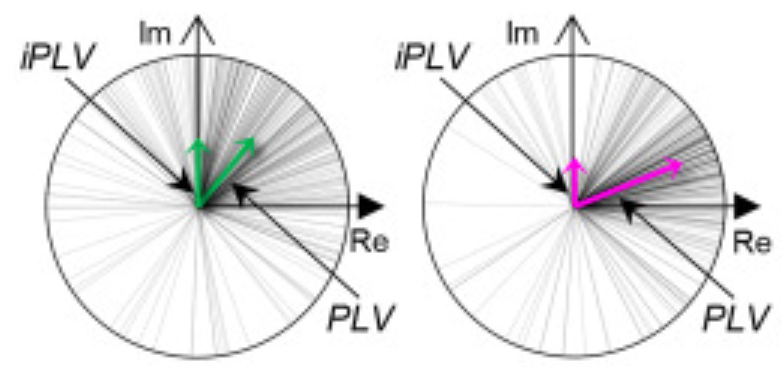
\includegraphics[scale=0.6]{14_1}
\end{figure}
This formulation allows to distinguish between the contributions due to volume conduction and the ones
related to connectivity. However, spurious connectivity can derive also from the fact that neurons are
locally connected and two brain regions may be connected via just a subset of the neurons that belong to
a narrow ensemble. The following model can be considered:
\begin{figure}[H]
    \centering
    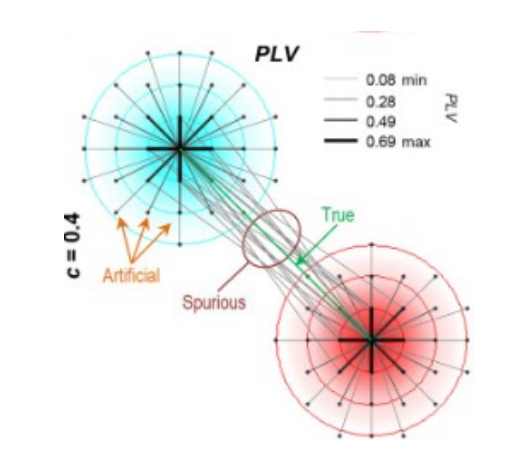
\includegraphics[scale=0.45]{14_2}
\end{figure}
Two brain regions are composed of many neurons among which just one is linked to the other area,
acting as a hub. Many electrodes are placed between these two areas and all the neurons in each area are
tightly connected together and exchange information. Since local connectivity is very fast, it can have
zero-lag components. Discarding them, also some elements related to the physiological activity can be
eliminated, thus the disadvantage of this approach is that it can cancel out also real genuine zero-lag
values.\\
On the other hand, this approach has the big advantage that its mathematical formulation is the same
seen before for the PLV, where instead of taking the absolute value of the PLV, the imaginary part and
then the absolute value are considered.\\
Another approach sometimes found in literature is the so-called Weighted Phase Lag Index, having a more
complex mathematical formulation w.r.t. the Imaginary PLV.

\subsection{Assessing Significance}
Independently of the way in which the connectivity profiles are looked at, it is important to understand
how to assess the actual significance of the observations that are carried out. The best way to do that
is by using a distribution under the null hypothesis. In the classical tests, it relies on the
assumption that data are distributed according to a Gaussian distribution. However, in such a case the
phase angles cannot be normally distributed as the statistic is circular, thus surrogate statistics need
to be built.\\
To do so, a circular rotation of one time serie with respect to the other is often employed: in this way,
the auto-correlation of one channel is maintained but the cross-correlation of two different channels is
disrupted as a consequence of the time rotation. This allows to observe the data under the null
hypothesis of no time correlation between different regions.
\subsubsection{An Algorithm to Test for Significance}
Since the recording is multi-channel, connectivity statistics such as PLV or any other pair-wise metric
can be computed. This will return the weighted \textbf{adjacency matrix}: a matrix in which the
connectivity between channels \(i\) and \(j\) is represented. Then, the surrogate statistics are calculated
and the null distribution is built.
\begin{figure}[H]
    \centering
    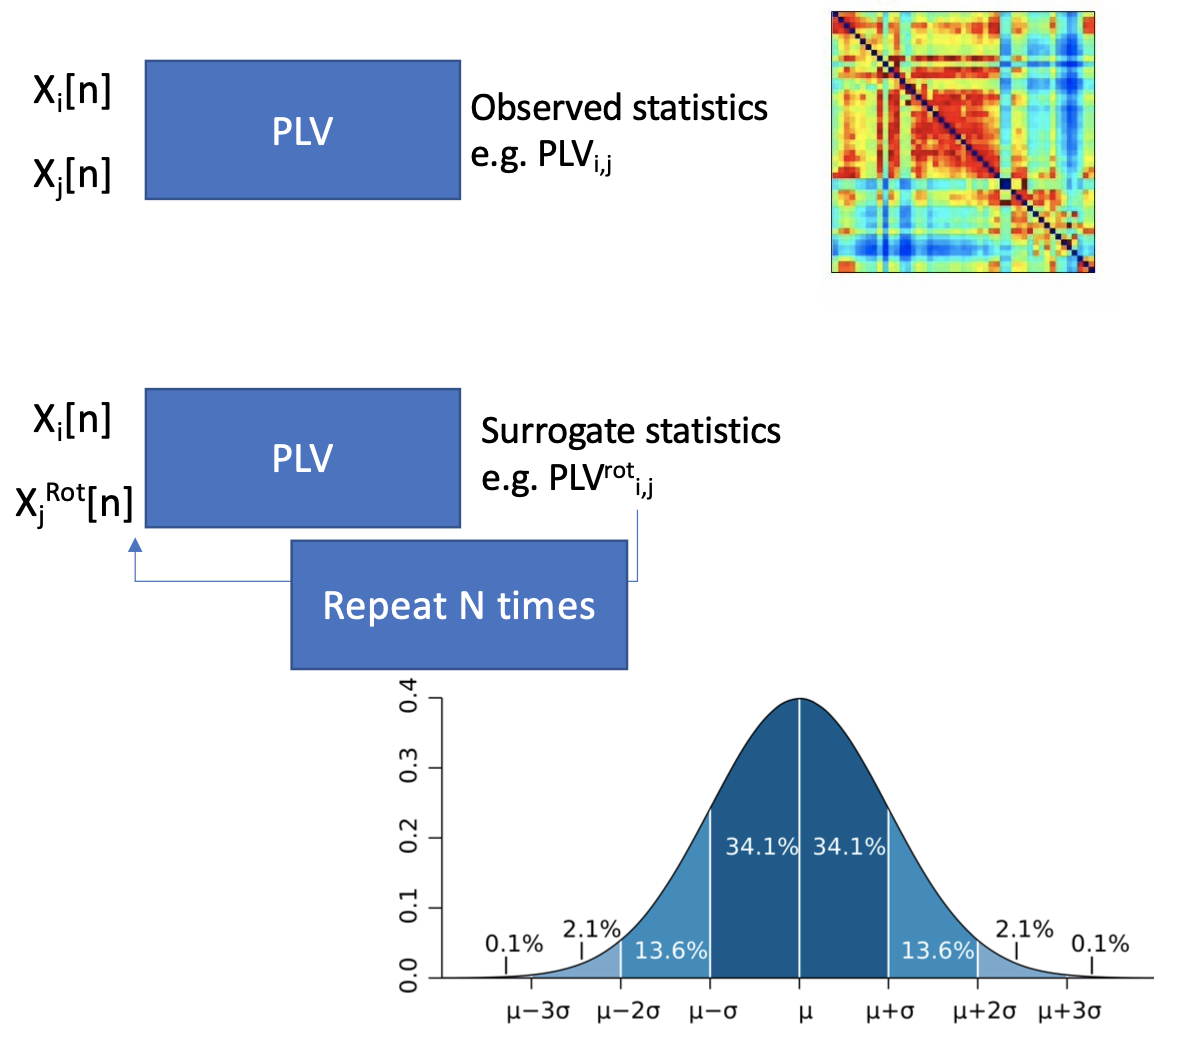
\includegraphics[scale=0.5]{14_3}
\end{figure}
To do this, the statistics are computed \(N\) times (the higher \(N\), the more reliable the statistics).
Every time the inputs of the statistics are slightly different: \(x_i\) remains the same but \(x_j\) is
randomly time-rotated. Hence, a more scattered and less clustered matrix is obtained. At this point, all
the new matrix values are picked and put in a histogram, whose distribution will resemble a Gaussian with
longer tails - i.e., a Rayleigh distribution -.\\
Any single element of the observed (experimental) matrix can be compared to the the p-value of the
probability density function. Then, the fraction of surrogate elements larger than a certain \(\alpha\)
value is taken into account. Thus, by filtering through the p-value, the number of channel pairs among
which the connection is significant can be counted.
\subsubsection{Results Visualization}
Different ways can be used to summarize the results:
\begin{itemize}
    \item \textbf{Spectrum of the connectivity:} the peaks describe characteristics of the activity,
          for instance by telling if it is physiological (like alpha synchronization).
    \item \textbf{Fraction of significance (\(K\)):} the number of elements significantly coupled in the
          considered network.
    \item \textbf{Adjacency matrix}
    \item \textbf{Brain plots:} each node represents one brain region and the edge connecting two nodes
          has a different intensity of color according to its PLV value.
\end{itemize}
\begin{figure}[H]
    \centering
    \subfigure[]{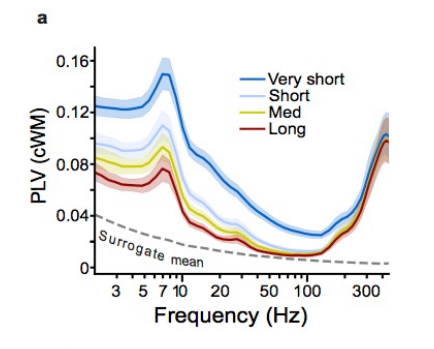
\includegraphics[width=0.3\textwidth]{14_4}}
    \subfigure[]{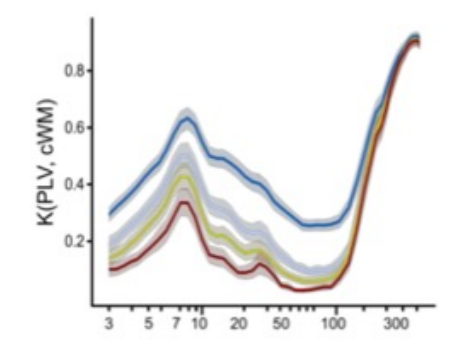
\includegraphics[width=0.3\textwidth]{14_5}}
\end{figure}
\begin{figure}[H]
    \centering
    \subfigure[]{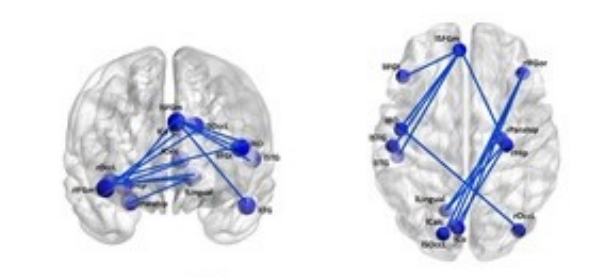
\includegraphics[width=0.4\textwidth]{14_6}}
    \subfigure[]{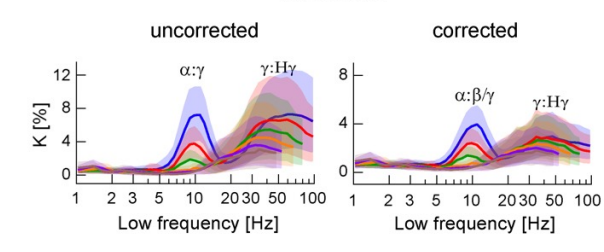
\includegraphics[width=0.5\textwidth]{14_7}}
\end{figure}

\subsection{Cross-Frequency Coupling}
The brain activity can be observed at different time, frequency, and spatial scales. Different
oscillations can be summed up together into a single field activity.
\begin{figure}[H]
    \centering
    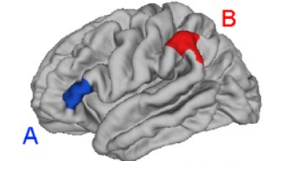
\includegraphics[scale=0.65]{14_8}
\end{figure}
The Cross-Frequency Coupling (CFC) is a communication mechanism between two different brain regions and is
related to the concept of communication coherence, stating that the membrane potential and the LFP
control the excitability of a cellular network. Consequently, if the electrical fields of two regions
oscillate with a constant time delay (in cross-connection), the probability of one stimulus to be
transmitted from one area to the other is strongly connected to the time delay of these two excitability
cycles of oscillations. Therefore, if the activity signal reaches the target region within its optimal
excitability cycle, the probability of communication is increased.\\
Neurons fire at higher frequencies than the field activity, as a consequence a spikes cannot be directly
measured through the field activity, it can only be assumed that the connectivity of slow oscillations
is representative of the excitability cycle or the CFC can be considered instead.
\begin{figure}[H]
    \centering
    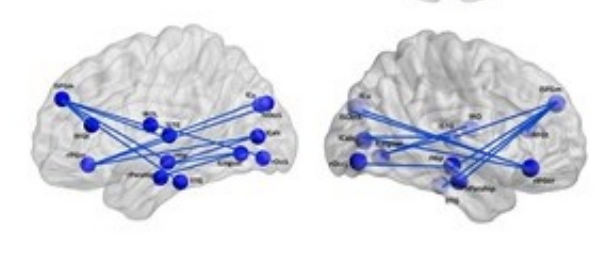
\includegraphics[scale=0.55]{14_9}
\end{figure}
The CFC attempts to measure the combination of phase and amplitude synchronization. Through this value,
the probability of communication by looking at the phase of the slow oscillations in connection with
the amplitude of the fast oscillations can be quantified. Every time the slow oscillations are
synchronized, there is an amplitude increase in the high oscillations representing an increase in the
firing activity. The CFC can be measured in multiple ways:
\begin{itemize}
    \item \textbf{PAC (Phase-Amplitude Coupling)}: this index looks at the correlation between
          synchronization of the slow rhythms and the co-increase of the amplitude oscillations.
          \begin{figure}[H]
              \centering
              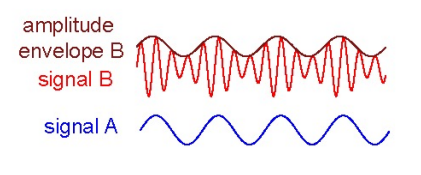
\includegraphics[scale=0.75]{14_10}
          \end{figure}
    \item \textbf{CFS (Cross-Frequency phase-phase Synchrony)}: this metric measures the coexistence of
          different oscillations and their relative space difference. Hence, it looks at the phase
          synchronization between two different rhythms.
          \begin{figure}[H]
              \centering
              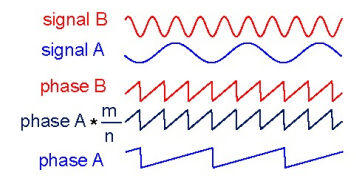
\includegraphics[scale=0.75]{14_11}
          \end{figure}
\end{itemize}

\subsection{The PAC Algorithm}
Given two signals \(A\) and \(B\) recorded at two different sites of the brain:
\begin{enumerate}
    \item Filter \(A\) in a LF range (\(2\,Hz\)) with the complex Morlet, such that the phase-time
          series can be extracted.
    \item Filter \(B\) in a HF range (\(120\,Hz\)) with the complex Morlet.
    \item To match together the two complex time series that have been found, the envelope from the
          filtered \(B\) is extracted (in order to look at the amplitude increase implying that the local
          neurons under the probe are actively doing something).\\
          Now, a phase time series and an amplitude time series that exist at the same time are obtained,
          so the PAC can be computed. Also, the amplitude envelope contains spurious noise and needs to
          be filtered. It can be done with the same LF filter used for signal \(A\). In this way,
          a specific amplitude modulation is considered, existing in the same frequency range of the
          slow oscillations, thus the noisy fast oscillations are being discarded.
    \item Compute the PLV. Instead of doing it between two different channels within the same band,
          the phases of steps \textbf{1.} and \textbf{3.} are to be employed. In this way, the phase
          synchronization between two different regions and two different frequency bands can be obtained
          by looking at how the phase of slow oscillations modulates the amplitude increase.
\end{enumerate}
\begin{figure}[H]
    \centering
    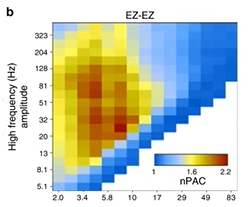
\includegraphics[scale=1.1]{14_12}
\end{figure}
If the algorithm is reapplied for different pairs of frequencies, the plot reported above can be drawn,
where on the axes there are the low and the high frequency ranges. Each element represents the average
of the phase-amplitude coupling. There are no elements in a part of the matrix as the phase modulation
of the high frequency with the amplitude modulation of the low frequency is not looked at, because that
would be physiologically not feasible.\\
Henceforth, this matrix shows how the different rhythms interact with each other forming a complex
network and allows to quantify how much the phase of one channel changes the amplitude of another
channel. For example, a phase-amplitude coupling in the hippocampus between theta and gamma oscillations
is well-described in literature.\\
\paragraph{What does an increase in PLV or PAC mean from a physiological point of view?}
Literature suggests that some increase in synchronization can be representative of neuro-degenerative
processes or pathological states, like epilepsy. An increase in phase synchronization of the theta band
is linked to the successfully recall of a memory from a memory task.

\subsection{Interaction Metrics}
\subsubsection{Coherence}
Coherence is the ratio between the cross-spectrum and the product of the auto-spectra of the two signals. It represents the linear spectral correlations between the two
signals, thus it cannot capture correlations that are not linear. It is sensitive to mixing factors - i.e., volume conduction -, hidden sources (bivariate method), and
common reference problems. An increase in coherence might either represent an increase in phase coherence or in amplitude correlation: these two elements cannot be
separated by just looking at the coherence value.\\
This value allows a bivariate analysis, in which the correlation between two regions is computed. The problem is that there are also spurious connections among them,
not only significant ones.
\subsubsection{Partial Coherence}
The first attempt to expand the bivariate analysis has been the addition of a third channel to the estimation of coherence. The main issue is that this method is very
sensitive to the SNR: if the SNR is not uniform in the 3 nodes, a stronger partial coherence can be estimated in the wrong side of the network. Furthermore, directional
connectivity cannot be distinguished.
\subsubsection{Granger Causality}
It is useful for understanding directional communication. It is based on the estimation of an Auto-Regressive model and it measures only the linear dependency between
two variables: its value is comprised between 0 and 1. It is based on the assumption that if the outcome of a variable \(X\) can be easily predicted by introducing
\textit{a priori} knowledge of \(X\) and \(Y\), then \(Y\) drives \(X\). This is not a real causality, but in some way it gives a directional information a bit larger
than the PLV.\\
However, this algorithm suffers an increase in the complexity required to estimate the parameters.
\subsubsection{Multivariate Methods}
The majority of these methods rely on Auto-Regressive (AR) models. The AR coefficients are derived such that the corresponding linear combination of the past values
of the signal provides the best (in the least squares sense) linear prediction of the current value. In practice, the MVAR method is a way to estimate these coefficients
and use them to compute various interaction measures. The solution of MVAR outputs is a linear time-invariant system (LTI), which imposes limitations when applied to an
obviously non-linear system as the human brain. Additionally, LTI imposes that the probability density function of the LTI output is a Gaussian.\\
Keep in mind that if the original data are convolved with a temporal filter, in most cases they will not follow an AR model due to the moving average term introduced by
such filtering.
\subsubsection{Partial Directed Coherence and Direct Transfer Function}
They are based on the estimation of a Multivariate Auto-Regressive (MVAR) model with the same criteria applied to the Granger Causality estimation.\\
As all the methods based on model fitting, the efficiency of these methods is strictly dependent on the selection of initial parameters. This indeed suggests to be
extremely careful on the decision of the optimal model order and epoch length.\\
The causality estimated by means of GC, PDC, and DTF methods is meaningful only in a statistical sense, because their computation depends completely on an estimation
of the model parameters. Also, preprocessing steps can lead to very different results and interpretations.
\subsubsection{Mutual Information}
The Mutual Information (MI) metric can be very interesting to look at when referred to spike analysis. As a matter of fact, an increase in the MI is associated with an
increase in communicability. On the other hand, the MI in the local field context is very complex to interpret. The problem with this type of metric is the computational
cost, as it is considerably high.
